\documentclass{standalone}
\usepackage{tikz}
\usepackage{ctex,siunitx}
\usepackage{tkz-euclide}
\usepackage{amsmath}
\usetikzlibrary{patterns, calc}
\usetikzlibrary {decorations.pathmorphing, decorations.pathreplacing, decorations.shapes,}
\begin{document}
\small
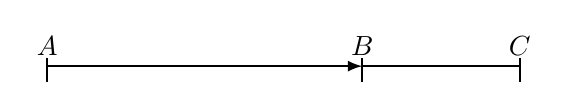
\begin{tikzpicture}[>=latex, thick]
  \draw [->](0,0)node[above]{$A$} --(4,0)node [above]{$B$} ;
  \draw (4,0)--(6,0)node [above]{$C$};
  \foreach \x in {0,4,6}
  {
    \draw (\x, -.2)--(\x,.1);
  }
\end{tikzpicture}
\end{document}